%set margins according to print 

\documentclass[a4paper,12pt]{book}
\setlength{\oddsidemargin}{ 0 in}
\setlength{\evensidemargin}{ 0 in}
\setlength{\topmargin}{-0.6 in}
\setlength{\textwidth}{6.5 in}
\setlength{\textheight}{8.5 in}
\setlength{\headsep}{0.75 in}
\setlength{\parindent}{0 in}
\setlength{\parskip}{0.1 in}

%packages list

\usepackage{amsmath,amsfonts,graphicx}
\usepackage{pgf,tikz}
\usepackage{subfig}
\usepackage{mathrsfs}
\usetikzlibrary{arrows}
\usepackage{pgfplots}
\pgfplotsset{dstyle/.style={xmin=-5,xmax=5,ymin=-2,ymax=2,xlabel=$n$,ylabel={$x[n]$},axis lines=center,samples=20,title=Discrete time,every axis x label/.style={at={(current axis.right of origin)},anchor=west},
every axis y label/.style={at={(current axis.north)},above=2mm}}}
\pgfplotsset{cstyle/.style={xmin=-5,xmax=5,ymin=-2,ymax=2,xlabel=$t$,ylabel={$x(t)$},axis lines=center,samples=100,title=Continuous time,every axis x label/.style={at={(current axis.right of origin)},anchor=west},
every axis y label/.style={at={(current axis.north)},above=2mm}}}
\pgfplotsset{
    dirac/.style={
        mark=triangle*,
        mark options={scale=2},
        ycomb,
        scatter,
        visualization depends on={y/abs(y)-1 \as \sign},
        scatter/@pre marker code/.code={\scope[rotate=90*\sign,yshift=-2pt]}
    }
}
%
% The following commands set up the lecnum (lecture number)
% counter and make various numbering schemes work relative
% to the lecture number.
%
\newcounter{lecnum}
\renewcommand{\thepage}{\thelecnum-\arabic{page}}
\renewcommand{\thesection}{\thelecnum.\arabic{section}}
\renewcommand{\theequation}{\thelecnum.\arabic{equation}}
\renewcommand{\thefigure}{\thelecnum.\arabic{figure}}
\renewcommand{\thetable}{\thelecnum.\arabic{table}}

%
% The following macro is used to generate the header.
%
\newcommand{\RNum}[1]{\uppercase\expandafter{\romannumeral #1\relax}}

\newcommand{\lecture}[4]{
   \pagestyle{myheadings}
   \thispagestyle{plain}
   \newpage
   \setcounter{lecnum}{#1}
   \setcounter{page}{1}
   \noindent
   \begin{center}
   \framebox{
      \vbox{\vspace{2mm}
    \hbox to 6.28in { {\bf B.Tech ECE: Signals and Systems
		\hfill \RNum{2}-\RNum{1} Semester} }
       \vspace{4mm}
       \hbox to 6.28in { {\Large \hfill Chapter #1: #2  \hfill} }
       \vspace{2mm}
       \hbox to 6.28in { {\it Lecturer: #3 \hfill Scribes: #4} }
      \vspace{2mm}}
   }
   \end{center}
   \markboth{Lecture #1: #2}{Lecture #1: #2}
   {\bf Disclaimer}: {\it These notes have not been subjected to the
   usual scrutiny reserved for formal publications.  They may be distributed
   outside this class only with the permission of the Lecturer.}
   \vspace*{4mm}
}
%
% Convention for citations is authors' initials followed by the year.
% For example, to cite a paper by Leighton and Maggs you would type
% \cite{LM89}, and to cite a paper by Strassen you would type \cite{S69}.
% (To avoid bibliography problems, for now we redefine the \cite command.)
% Also commands that create a suitable format for the reference list.
\renewcommand{\cite}[1]{[#1]}
\def\beginrefs{\begin{list}%
        {[\arabic{equation}]}{\usecounter{equation}
         \setlength{\leftmargin}{2.0truecm}\setlength{\labelsep}{0.4truecm}%
         \setlength{\labelwidth}{1.6truecm}}}
\def\endrefs{\end{list}}
\def\bibentry#1{\item[\hbox{[#1]}]}

%Use this command for a figure; it puts a figure in wherever you want it.
%usage: \fig{NUMBER}{SPACE-IN-INCHES}{CAPTION}
\newcommand{\fig}[3]{
			\vspace{#2}
			\begin{center}
			Figure \thelecnum.#1:~#3
			\end{center}
	}



% Use these for theorems, lemmas, proofs, etc.
\newtheorem{theorem}{Theorem}[lecnum]
\newtheorem{lemma}[theorem]{Lemma}
\newtheorem{proposition}[theorem]{Proposition}
\newtheorem{claim}[theorem]{Claim}
\newtheorem{corollary}[theorem]{Corollary}
\newtheorem{definition}[theorem]{Definition}
\newenvironment{proof}{{\bf Proof:}}{\hfill\rule{2mm}{2mm}}

\begin{filecontents*}{datafile.dat}
-5        -0.03
-4        0.0625
-3        -0.125
-2        0.25
-1        -0.5
0        0.0
1        -2
2        4
3        -8
4        16
5        -32

\end{filecontents*}

\begin{document}
\title{\Large{\textbf{Signals and Systems}}}
\author{By Shriram R}
\date{August 2019}
\maketitle
\let\cleardoublepage\clearpage
\tableofcontents
\chapter{Signal Analysis}
%\lecture{**LECTURE-NUMBER**}{**DATE**}{**LECTURER**}{**SCRIBE**}
\lecture{1}{Signal Analysis}{Syed Munavvar Hussain}{Shriram R}
%\footnotetext{These notes are partially based on those of Nigel Mansell.}

% **** YOUR NOTES GO HERE:

Signals can be used to describe a wide range of natural phenomena. A signal is generally imagined as a pattern of variations of some quantity with respect to another independent quantity. In the following section we shall look into the definition of a signal as well as a system along with some examples

\section{Introduction} 

\begin{description}
	\item[Signal] It is defined as a function of any independent variable. Generally speaking, a signal is a function of time which conveys some sort of information.\\
\textbf{E.g;}
\begin{itemize}
\item Speech or Voice signals
\item Image signals 
\item etc
\end{itemize}
\item[System] It is a collection of objects which work together to perform a particular task.\\
From a communications standpoint, systems are used to process signals.
\end{description}

\section{Classification of Signals}
If a signal is defined in terms of only one independent variable, it is called a one dimensional signal otherwise it is called a multi-dimensional signal.\\
in addition to dimensions,signals can be classified on the basis of various parameters:
\subsection*{\Large{On the basis of time $t$}}
\textbf{Continuous Time Signals}\\
A signal which is defined continuously for all values of time $t$ is called a continuous time signal. It is represented by $x(t)$ (in parentheses) and are also called analog signals.

{\bf Discrete Time Signals}\\ A signal that is defined for only specific instances of time or at discrete values of time.It is represented by $x[n]$ (in brackets).It is generally obtained by sampling an analog signal.\\

{\bf These signals can be further classified as follows:}
\subsection*{\Large{On the basis of periodicity}}
\textbf{Periodic Signals :}
{\bf Continuous Time Periodic Signals }\\
a signal is said to be CT-periodic if it repeats after a certain time interval $T_0$\\
Mathematically, it is defined as the signal which satisfies :\\
\begin{align*}
x(t)=x(t+T_0)  \forall  t  \in R
\end{align*}
{\bf Discrete Time Periodic Signals }\\
a signal is said to be DT-periodic if it repeats after a certain time interval $N_0$\\
Mathematically, it is defined as the signal which satisfies :\\
\begin{align*}
x[n]=x[n+N_0]  \forall  n  \in Z
\end{align*}
{\bf Aperiodic Signals :}\\ A signal that does not satisfy the above conditions is called aperiodic signal. It may be viewed as a limiting case of a periodic signal in which period tends to Infinity.
\subsection*{\Large{Even and Odd signals }}
	a signal $x(t)$ is said to be even if it satisfies :
	\begin{align*}
	x(t)=x(-t){\hspace{4mm}(CT)}\\
	x[n]=x[-n]{\hspace{4mm}(DT)}
	\end{align*}
	a signal x(t) is said to be odd if it satisfies :
	\begin{align*}x(t)=-x(-t){\hspace{4mm}(CT)}\\x[n]=-x[-n]{\hspace{4mm}(DT)}\end{align*}	
	if it satisfies neither it is said to be neither even nor odd.\\

\subsection*{\Large{Deterministic and Random Signals }}
A signal is said to be deterministic if there is no uncertainty with respect to its value at any instant of time. Or, signals which can be defined exactly by a mathematical formula are known as deterministic signals.\\

A signal is said to be non-deterministic if there is uncertainty with respect to its value at some instant of time. Non-deterministic signals are random in nature hence they are called random signals. Random signals cannot be described by a mathematical equation. They are modelled in probabilistic terms.\\
\subsection*{\Large{Energy and Power Signals }}
A signal is said to be energy signal when it has finite energy.
$$\text{Energy}\, E = \int_{-\infty}^{\infty} |x\,(t)|^2dt$$
A signal is said to be power signal when it has finite power.
$$\text{Power}\, P = \lim_{T \to \infty}\,{1\over2T}\,\int_{-T}^{T}\,|x(t)|^2dt$$
NOTE:A signal cannot be both, energy and power simultaneously. Also, a signal may be neither energy nor power signal.

\begingroup
\centering

Power of energy signal = 0\\
Energy of power signal =$\infty$

\endgroup
\pagebreak
\section{Standard Signals}
There are some standard signals which are used repeatedly in signals and systems. Let us take a look on some of them.\vspace{4mm}\\
{\bf Standard signals list:}
\begin{enumerate}
\item Unit step signal
\item Unit Ramp signal
\item Unit parabolic
\item Signum
\item Real And Complex Exponential Signals
\item Sinusoidal Signals
\item Rectangular Signals
\item Triangular signal
\item Sampling Function
\item Sinc Function
\item Gaussian Pulse
\item Unit Impulse
\end{enumerate}

\subsection*{Unit step signal}
{\bf for continuous time :}\\
	\[ x(t) = \left\{ \begin{array}{ll}

	1 & \mbox{if $t > 0$;} \\

	0 & \mbox{if $t < 0$;} \\

	\end{array}
	\right. \]
at t=0 there is a discontinuity. but generally it can be said that the value converges to 0.5.\\
\bigskip
{\bf for discrete time :}\\
	\[ x[n] = \left\{ \begin{array}{ll}

	1 & \mbox{if $n \geq 0$;} \\

	0 & \mbox{if $n < 0$;} \\

	\end{array}
	\right. \]

\begin{figure}[h]  
\centering 
\begin{tikzpicture}[scale=0.7]
            \begin{axis}[cstyle]
                \addplot[smooth,black,thick] {0.5*(x/abs(x)+1)};
            \end{axis}
        \end{tikzpicture}\hspace{6mm}
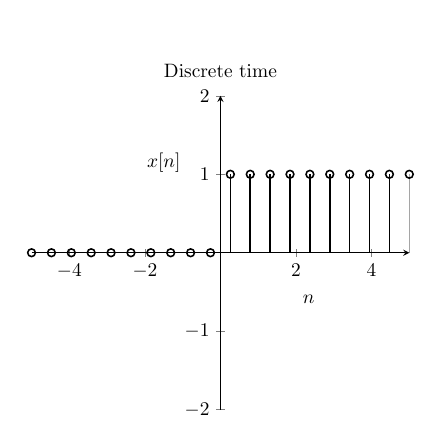
\begin{tikzpicture}[scale=0.7]
            \begin{axis}[dstyle]
                \addplot+[ycomb,black,thick,mark=o] {0.5*(x/abs(x)+1)};
            \end{axis}
        \end{tikzpicture}
\caption{the unit step signal} \label{fig:M}  
\end{figure}

\subsection*{ Ramp signal}
{\bf for continuous time :}\\
	\[ x(t) = \left\{ \begin{array}{ll}

	t & \mbox{if $t > 0$;} \\

	0 & \mbox{if $t < 0$;} \\

	\end{array}
	\right. \]
\bigskip
{\bf for discrete time :}\\
	\[ x[n] = \left\{ \begin{array}{ll}

	n & \mbox{if $n \geq 0$;} \\

	0 & \mbox{if $n < 0$;} \\

	\end{array}
	\right. \]

{\bf note:} The ramp signal can be related to the unit step by the following relation :

\begin{align*}
\frac{d }{dt}r(t) = u(t)
\end{align*}

\begin{figure}[h]  
\centering 
\begin{tikzpicture}[scale=0.7]
            \begin{axis}[cstyle]
                \addplot[smooth,black,thick] {x*(0.5*(x/abs(x)+1))};
            \end{axis}
        \end{tikzpicture}\hspace{6mm}
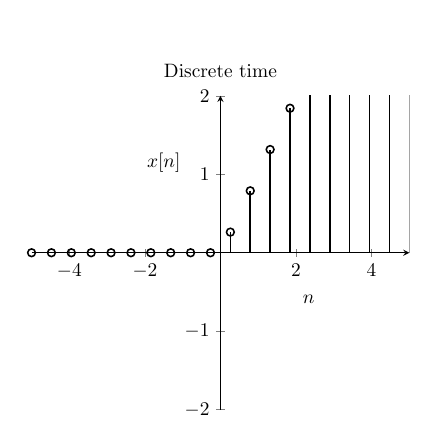
\begin{tikzpicture}[scale=0.7]
            \begin{axis}[dstyle]
                \addplot+[ycomb,black,thick,mark=o] {x*(0.5*(x/abs(x)+1))};
            \end{axis}
        \end{tikzpicture}
\caption{the ramp signal} \label{fig:M}  
\end{figure}

\subsection*{ Parabolic signal}
{\bf for continuous time :}\\
	\[ x(t) = \left\{ \begin{array}{ll}

	\frac{t^2 }{2} & \mbox{if $t > 0$;} \\

	0 & \mbox{if $t < 0$;} \\

	\end{array}
	\right. \]
\bigskip
{\bf for discrete time :}\\
	\[ x[n] = \left\{ \begin{array}{ll}

	\frac{n^2 }{2} & \mbox{if $n \geq 0$;} \\

	0 & \mbox{if $n < 0$;} \\

	\end{array}
	\right. \]

{\bf note:} The parabolic signal can be related to the ramp signal by the following relation :

\begin{align*}
\frac{d }{dt}p(t) = r(t)
\end{align*}

\begin{figure}[h]  
\centering 
\begin{tikzpicture}[scale=0.7]
            \begin{axis}[cstyle]
                \addplot[smooth,black,thick] {0.5*x^2*(0.5*(x/abs(x)+1))};
            \end{axis}
        \end{tikzpicture}\hspace{6mm}
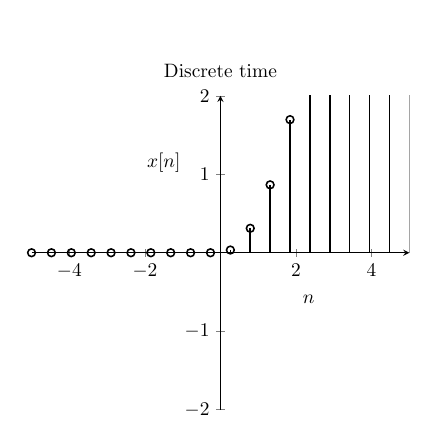
\begin{tikzpicture}[scale=0.7]
            \begin{axis}[dstyle]
                \addplot+[ycomb,black,thick,mark=o] {0.5*x^2*(0.5*(x/abs(x)+1))};
            \end{axis}
        \end{tikzpicture}
\caption{the parabolic signal} \label{fig:M}  
\end{figure}

\subsection*{ signum function}
{\bf for continuous time :}\\
	\[ x(t) = \left\{ \begin{array}{ll}

	1 & \mbox{if $t > 0$;} \\

	0 & \mbox{if $t = 0$;} \\
	-1 & \mbox{if $t < 0$;}
	\end{array}
	\right. \]
\bigskip
{\bf for discrete time :}\\
	\[ x[n] = \left\{ \begin{array}{ll}

	1 & \mbox{if $t > 0$;} \\

	0 & \mbox{if $t = 0$;} \\
	-1 & \mbox{if $t < 0$;}

	\end{array}
	\right. \]

{\bf note:} signum can be related to the unit step signal by the following relation :
\begin{align*}
u(t) = \frac{1}{2}(sgn(t)-1)
\end{align*}

\begin{figure}[h]  
\centering 
\begin{tikzpicture}[scale=0.7]
            \begin{axis}[cstyle]
                \addplot[smooth,black,thick] {(x/abs(x))};
            \end{axis}
        \end{tikzpicture}\hspace{6mm}
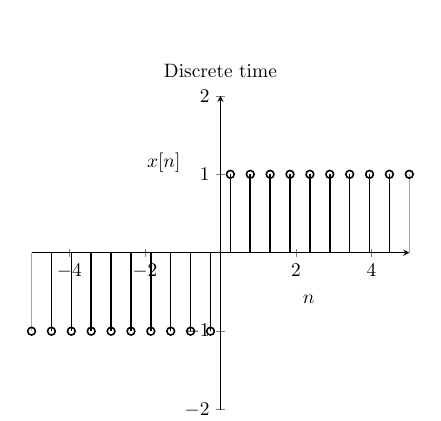
\begin{tikzpicture}[scale=0.7]
            \begin{axis}[dstyle]
                \addplot+[ycomb,black,thick,mark=o] {x/abs(x)};
            \end{axis}
        \end{tikzpicture}
\caption{Signum Function} \label{fig:M}  
\end{figure}

\subsection*{ Real Exponential signal}
{\bf for continuous time :}\smallskip\\
	 $x(t) = Ca^t$ \hspace{4mm} for $a>0$\\
\bigskip\\
{\bf for discrete time :}\smallskip\\
	$x[n] = Ca^n$\hspace{4mm} for $a>0$\\

\begin{figure}[h]  
\centering 
\begin{tikzpicture}[scale=0.7]
            \begin{axis}[cstyle,title=growing]
                \addplot[smooth,black,thick] {2.71828^x};
            \end{axis}
        \end{tikzpicture}\hspace{6mm}
\begin{tikzpicture}[scale=0.7]
            \begin{axis}[cstyle,title=Decaying]
                \addplot[smooth,black,thick] {2.71828^(-x)};
            \end{axis}
        \end{tikzpicture}
\caption{real exponential signal} \label{fig:M}  
\end{figure}

\subsection*{ Complex Exponential signal}
{\bf for continuous time :}\smallskip\\
	 $x(t) = Ca^t$ \hspace{4mm} for $a<0$\\
\bigskip\\
{\bf for discrete time :}\smallskip\\
	$x[n] = Ca^n$\hspace{4mm} for $a<0$\\


\begin{figure}[h]  
\centering 
\begin{tikzpicture}[scale=0.7]
            \begin{axis}[axis lines = center,title=discrete time]
                \addplot+[ycomb,black] plot table[y index=1]{datafile.dat};
            \end{axis}
        \end{tikzpicture}\hspace{4mm}
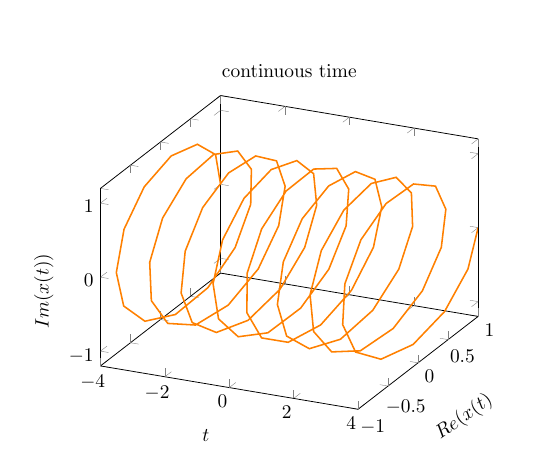
\begin{tikzpicture}[scale=0.7]
            \begin{axis}[xlabel=$t$,ylabel=$Re(x(t)$,zlabel=$Im(x(t))$, y label style={rotate = 35},title=continuous time]
               \addplot3[
            y domain=0:0,
            orange,samples=100,
            domain=-4:4,thick
            ]
            ({x},{cos(deg(2*pi*x))},{sin(deg(2*pi*x))});
            \end{axis}
        \end{tikzpicture}
\caption{complex exponential signal} \label{fig:M}  
\end{figure}

\subsection*{Sinusoidal signals}
{\bf for continuous time :}\\
	 $$ x(t) = sin(\omega_0 t+ \theta)$$ \\
where, $\omega_0 = \frac{2\pi}{T_0}$ is the fundamental frequency and $\theta$ is the phase.\\
\begin{figure}[h]  
\centering 
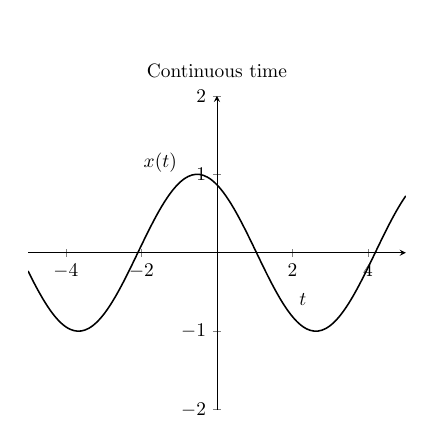
\begin{tikzpicture}[scale=0.7]
            \begin{axis}[cstyle]
                \addplot[smooth,black,thick] {cos(x*180/pi + 30)};
            \end{axis}
        \end{tikzpicture}
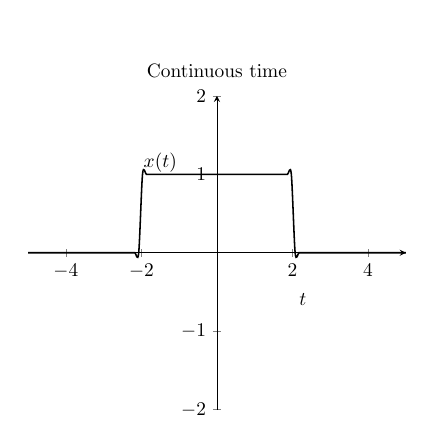
\begin{tikzpicture}[scale=0.7,
	declare function={
    func(\x)= (\x < -2) * (0)   +
              and(\x >= -2, \x < 2 ) * (1)     +
              (\x >= 2) * (0);
  }]
	
            \begin{axis}[cstyle]
                \addplot[smooth,black,thick] {func(x)};
            \end{axis}
        \end{tikzpicture}
\caption{a sinusoid and rectangular signal} \label{fig:M}  
\end{figure}

\subsection*{ Rectangular signal a.k.a Gating pulse}
{\bf for continuous time :}\\
	\[ x(t) = \left\{ \begin{array}{ll}

	A & \mbox{if $\frac{-T}{2}< t <\frac{T}{2}$;} \\

	0 & \mbox{otherwise} \\
	\end{array}
	\right. \]
\pagebreak

\subsection*{Triangular pulse}
{\bf for continuous time :}\\
	\[ x(t) = \left\{ \begin{array}{ll}

	\frac{A}{T}t+A & \mbox{if $ T \leq t \leq 0$;} \\

	\frac{-A}{T}t+A & \mbox{if $0 \leq t \leq T$;} \\

	\end{array}
	\right. \]
\begin{figure}[h]  
\centering 
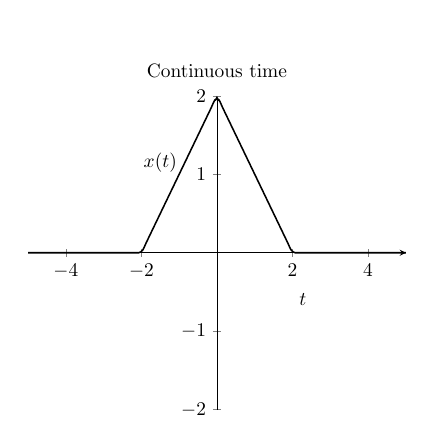
\begin{tikzpicture}[scale=0.7,
	declare function={
    func(\x)= (\x < -2) * (0)   +
              and(\x >= -2, \x < 2 ) * (2-abs(x))     +
              (\x >= 2) * (0);
  }]
	
            \begin{axis}[cstyle]
                \addplot[smooth,black,thick] {func(x)};
            \end{axis}
        \end{tikzpicture}
\caption{Triangular pulse} \label{fig:M}  
\end{figure}

\subsection*{Sampling function $Sa(t)$}
{\bf for continuous time :}\\
	$$Sa(t) =\frac{sin(t)}{t} \hspace{4mm}\forall t \in R $$
\bigskip\\

\subsection*{Sinc function $Sinc(t)$}
The sinc function is a time scaled version of the sampling function. specifically , the time variable t is scaled as $$t \longrightarrow \pi t$$
The full name of the function is "sine cardinal," but it is commonly referred to by its abbreviation, "sinc."\\ It is a function that arises frequently in signal processing and the theory of Fourier transforms.\\
{\bf for continuous time :}\\
	$$Sinc(t) =\frac{sin(\pi t)}{\pi t} \hspace{4mm} \forall t \in R $$ \\
	it may also be defined as:
	$$sinc(t)=Sa(\pi t)$$
\begin{figure}[h]  
\centering 
\begin{tikzpicture}[scale=0.7]
            \begin{axis}[cstyle]
                \addplot[smooth,black,thick] {sin(x*180/pi)/x};
            \end{axis}
        \end{tikzpicture}\hspace{5mm}
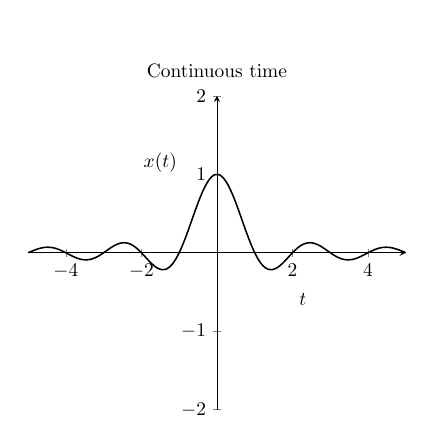
\begin{tikzpicture}[scale=0.7]
            \begin{axis}[cstyle]
                \addplot[smooth,black,thick] {sin(x*180)/(pi*x)};
            \end{axis}
        \end{tikzpicture}
\caption{Sampling and Sinc functions} \label{fig:M}  
\end{figure}
\pagebreak
\subsection*{Gaussian Pulse}
{\bf for continuous time :}\\
	$$x(t) =e^{-at^2} \hspace{4mm} \forall t \in R $$ \\
\begin{figure}[h]  
\centering 
\begin{tikzpicture}[scale=0.7]
            \begin{axis}[cstyle]
                \addplot[smooth,black,thick] {e^(-x^2)};
            \end{axis}
        \end{tikzpicture}
\caption{Gaussian Pulse} \label{fig:M}  
\end{figure}
	
\subsection*{Impulse signal}
The Impulse signal in continuous time is also called the 'Dirac Delta'. It is represented by $\delta(t)$.\\
formally, the defintion for this function is : $$\int_{-\infty}^{\infty}\delta (t)dt = 1$$

{\bf for continuous time :}\\
	\[ x(t) = \left\{ \begin{array}{ll}

	$$\infty$$ & \mbox{for $t = 0$;} \\

	0 & \mbox{otherwise;} \\

	\end{array}
	\right. \]
\bigskip
In discrete time, it is called the Kronecker delta or 'Unit impulse'.
{\bf for discrete time :}\\
	\[ x[n] = \left\{ \begin{array}{ll}

	1 & \mbox{if $n = 0$;} \\

	0 & \mbox{otherwise} \\

	\end{array}
	\right. \]

\begin{figure}[h]  
\centering 
\begin{tikzpicture}[scale=0.7]
            \begin{axis}[cstyle]
                \addplot[dirac] coordinates {(1,1)};
            \end{axis}
        \end{tikzpicture}\hspace{6mm}
\begin{tikzpicture}[scale=0.7]
            \begin{axis}[dstyle]
                \addplot+[ycomb,red,thick,mark=o] coordinates {(1,1)};
            \end{axis}
        \end{tikzpicture}
\caption{$\delta(t-1)$} \label{fig:M}  
\end{figure}
{\bf Note:}\\
\begin{itemize}
\item the unit impulse is the first difference of the unit step sequence.
$$\delta[n]=u[n]-u[n-1]$$
\item alternatively:
$$u[n]=\sum_{n=-\infty}^{+\infty}\delta[n]$$
\item the dirac delta is the first derivative of the unit step signal.
$$\delta(t)=\frac{d}{dt}u(t)$$
\item alternatively:
$$u(t)=\int_{-\infty}^{+\infty}\delta(t)$$
\end{itemize}
{\bf Properties of impulse signal:}\\
\begin{itemize}
\item The integral of the impulse over R is unity.
$$\int_{-\infty}^{\infty}\delta (t)dt = 1$$
\item Sifting\\
$$\int_{a}^{b}x(t)\delta(t-T)dt=\begin{cases}
x(T) for a<T<b;\\
0\hspace{4mm} otherwise;\\
\end{cases} $$
thus it can be imagined that the impulse function $\delta(t-T)$ sifts through the function f(t) and pulls out the value f(T).\\
\item Convolution and Sifting\\
Convolution of a function with a shifted impulse yields a shifted version of that function. whereas convolution of a function with an impulse at t=0 yields the function itself.
$$x(t) \ast \delta(t-T) = x(t-T)$$
\item Time scaling\\
The unit impulse time-scaled by a factor of a is the unit impulse amplitude-scaled by a factor of 1/|a|\\
$$\delta(at)=\frac{1}{a}\delta(t)$$
\item Similarly sifting in discrete time:\\
$$x[n_0] = \sum_{n = -\infty}^\infty \delta[n - n_0] x[n]$$
\item and convolution in discrete time:\\
$$x[n] \ast \delta[n-n_0] = x[n-n_0]  $$
\end{itemize}
\section{Next topic}
\begingroup
\centering


Here is how to define things in the proper mathematical style.
Let $f_k$ be the $AND-OR$ function, defined by

\[ f_k(x_1, x_2, \ldots, x_{2^k}) = \left\{ \begin{array}{ll}

	x_1 & \mbox{if $k = 0$;} \\

	AND(f_{k-1}(x_1, \ldots, x_{2^{k-1}}),
	   f_{k-1}(x_{2^{k-1} + 1}, \ldots, x_{2^k}))
	 & \mbox{if $k$ is even;} \\

	OR(f_{k-1}(x_1, \ldots, x_{2^{k-1}}),
	   f_{k-1}(x_{2^{k-1} + 1}, \ldots, x_{2^k}))	
	& \mbox{otherwise.} 
	\end{array}
	\right. \]
Here is a citation, just for fun~\cite{CW87}.
\section*{References}
pass
\end{document}





